\documentclass[12pt,a4paper]{report}

% Variables
\newcommand{\coursenumber}{02257}
\newcommand{\coursename}{Applied Functional Programming}
\newcommand{\projectnameshort}{Project 2}
\newcommand{\projectnamelong}{Project 2: \textit{Molecular Programming Language}}
\newcommand{\thedate}{\today}
\renewcommand\thesection{\arabic{section}}

\usepackage{newfloat}
\usepackage{syntax}
\usepackage[margin=25mm]{geometry}
\DeclareFloatingEnvironment[
  % the file extension for the file used to create the list:
  fileext   = logr,% don't use log here!
  % the heading for the list:
  listname  = {List of Grammars},
  % the name used in captions:
  name      = Grammar,
  % the default floating parameters if the environment is used
  % without optional argument:
  placement = htb
]{Grammar}
\usepackage[page,toc,titletoc,title]{appendix}

\usepackage{graphicx}
\usepackage{hyperref}
\usepackage{float}
\usepackage{listings}
\usepackage{xcolor}
\usepackage{parskip}
\usepackage{comment}
\usepackage{subcaption}
\setlength{\parindent}{0pt}

% Define the F# style
\lstdefinestyle{fsharpstyle}{
  basicstyle=\ttfamily\small,
  keywordstyle=\color{blue},
  commentstyle=\color{green!60!black},
  stringstyle=\color{purple},
  showstringspaces=false,
  numbers=left,
  numberstyle=\tiny,
  numbersep=5pt,
  tabsize=2,
  captionpos=b,
  frame=single,
  breaklines=true,
  breakatwhitespace=false,
  morekeywords={type, let, of, do, return, match, with},
}

% Set the default style to F#
\lstset{style=fsharpstyle}


\usepackage{biblatex}
\addbibresource{references.bib}

\begin{document}

\newgeometry{top=3.0cm}
\begin{titlepage}
    \begin{center}
        
\includegraphics[width=0.15\textwidth]{Report/frontmatter/dtu.pdf}\par\vspace{0.5cm}
    
        {\scshape\LARGE Technical University of Denmark\\}
    	\vspace{0.5cm}
        {\large \coursenumber\;\coursename}\\
    	\vspace{1.5cm}
    	{\huge\bfseries \projectnamelong\\}
    	\vspace{1.5cm}
    	{\Large Steffan Martin Kunoy (s194006)\\}
            {\Large Tjark Petersen (s186083)\\}
        \vspace{1cm}
    	{\Large \thedate\\}
        \vspace{1cm}

    \end{center}    
    \textbf{\textit{Abstract}}\\
        The CRN++ language presented by \citeauthor{soloveichik2018a} is a domain specific language to describe chemical reaction networks (CRN), which provide a basis for performing complex algorithmic computations in chemical solutions.
        
        In this report, we describe the F\# implementation of a parser and interpreter for the CRN++ language, a compiler which translates a CRN to a set of reactions and finally a chemical reaction simulator with a visualization backend which can be used to accurately simulate compiled CRNs. This is based on a thorough analysis of the CRN++ grammar, a definition of a well-formed CRN++ program and associated properties. Our implementation has been used to successfully compile and simulate a selection of example as well as randomly generated programs, with the output of the simulator being validated using the interpreter.
 \vfill
\end{titlepage}
\restoregeometry
\newpage


\tableofcontents
\thispagestyle{empty}
% possible todos:
% opt sim by only calculating concChange for non-catalysts (netchange != 0)


\begin{comment}
\begin{itemize}
    \item We changed the multiplicity of cmp molecules (such as xgty) from 1 to 2, because deactivated conditional reactions were else still too active
    \item The \texttt{sqrt} module for CRN++ returns the 4th root of the argument. As a result, we modified the interpreter output for the 
    \item Mul(a,b,c) is restricted further by a!=b
    \item Sub(a,b,c) is also restricted by a!=b
    \item debugging
    \begin{itemize}
        \item subhelper really high due to a < b in a-b and fall time too long when subhelper is used again
    \end{itemize}
\end{itemize}
\end{comment}

\newpage
\setcounter{page}{1}

\section{Introduction}
This report documents the design, implementation and testing of a tool for computing on the basis of chemical reaction networks (CRNs) using the functional programming language F\#. The project is inspired by the formalization of a language for chemical reactions proposed in \textit{CRN++: Molecular Programming Language} \cite{soloveichik2018a}. 

\section{CRN++}

\subsection{Revised Grammar} % Tjark

\subsection{Well-Formed CRN} % Steffan

\subsection{Abstract Syntax Tree Model} % Steffan
% F# type declarations
% Use DrawingTreesLib to draw example CRN++ program

\subsection{Parser for CRN++} % Tjark
% Parsed string property

\subsection{Type Checker for CRN++} % Steffan

\subsection{CRN Generator} % Tjark
% Define custom generator for FsCheck that produces well-formed CRNs

\subsection{CRN States}
% Representation of step outputs from chemical reactions

\subsection{Visualization} % Steffan

\section{Interpreter for CRN++}\label{sec:interpreter} % Steffan
% Initial state from conc
% Recurring steps application
When running a parsed CRN++ program using our interpreter, we generate an infinite sequence of \hyperref[sec:states]{CRN states}. The initial state is based on the collection of \texttt{conc} elements in the root of the program. Each subsequent state is synthesized by evaluating the commands in the next step of the program and updating the species concentrations accordingly. The application of steps is running in a loop, with the final step being immediately followed by the first step, and therefore the interpreter yields an infinite sequence of states.

%\subsection{Commutative property of step commands}
% used property based testing to verify that order of step commands does not matter
Our interpreter evaluates commands in the order given by the source code. This does of course not correspond to what would happen in the actual chemical reactions, where every operation depends on the newest \textit{stable} value in a step (under the assumption that enough time is given for all concentrations to reach steady state). Thus the order in which computations are written inside a step should not matter.

In principle the interpreter should be extended to order all commands in a step according to all dependency chains. This would lead to the evaluation of all dependencies of a command before it is evaluated itself. An attempt was made to implement this ordering using a dependency tree, but this proved difficult to implement given the time restrictions. We therefore instead expect the programmer to write commands in dependency order.

\section{Compiler for CRN++} % Tjark
% CRN -> list Reaction + initial concentrations
% Chemical clock oscillators
% flag molecules
% helper molecules

The ultimate purpose of the CRN++ language is to describe chemical reaction networks, so compiling the language involves the translation of the program into a sequence of reactions and a description of the initial concentrations of all the involved species. This provides the complete recipe to actually implement the CRN with concrete molecules. 

The translation from modules to reactions is based on what is described by \citeauthor{soloveichik2018a} \cite{soloveichik2018a}. The compiler consists of a collection of functions, each translating a certain level of the AST to reactions and possibly collecting the output of other compiler functions to achieve this task. In what follows, some of the key challenges and our solutions to them will be highlighted.

\subsection{Helper Species}
The subtraction reactions make use of a helper species $H$. Every subtraction running in parallel with other subtractions requires its own unique helper species for all subtractions to work properly. Since reactions only run in parallel within a step, helper species can be reused between steps. 

We chose to implement the handling of helper species in such a way that more reactions relying on helper species could easily be added. This involves maintaining a per step helper map, which maps a helper species name to an integer providing an instance count. This map is used to  enumerate helper species instances. The initial concentration for a helper species is collected in an initialization map.

\subsection{Sequential Execution}
Sequential execution in CRNs is enabled by a series of chemical oscillators which spike up one after the other and can be used as catalysts to activate reactions during their respective peaks. In practice, this means that all reactions collected inside a step have to add the clock species associated to this step on either side of their reaction equation. \citeauthor{soloveichik2018a} suggest to use every third peak for actual computation since there is some overlap between successive peaks. Thus $3\times \#Steps$ clock species are required in a CRN.

\citeauthor{soloveichik2018a} do not talk about how to initialize these clock species. It can be seen that each peak has a maximum concentration of 2. Since the oscillator CRN is a closed system and all other clock species have concentrations of close to 0 while another has its peak, the combined concentration of all clock species must be 2. Through experimenting, it was discovered that the initial distribution of $X_{n-1}=0.9$, $X_{0}=1.0$ and $X_i=10^{-10}$ for all other clock species gives an oscillation close to the natural frequency of the system.

Reactions in a step have access to the step number $i$ when creating the reaction equations and can bind their reactions to the species $X_{3i}$.

\subsection{Comparison and Conditional Execution}
Comparison operations in the CRN++ language rely on an implicit flag species which is set by \texttt{cmp} operations and used by conditional blocks. Since perfect equality is difficult to achieve according to \citeauthor{soloveichik2018a}, a $\pm \epsilon$ equality is used which actually compares $x+\epsilon$ and $y$ as well as $x$ and $y+\epsilon$. This results in four species: \texttt{xgty}, \texttt{xlty}, \texttt{ygtx} and \texttt{yltx} where the first species is offset by $\epsilon$. A table of how these species are used as catalysts for certain conditional blocks is shown in the following:

\begin{center}
\begin{tabular}{c|c|c|c|c}
    \texttt{IfGT} & \texttt{IfGE} & \texttt{IfEQ} & \texttt{IfLE} & \texttt{IfLT} \\\hline
    $2\times\:$\texttt{xgty} & \texttt{xgty} & \texttt{xgty} & \texttt{ygtx} & $2\times\:$\texttt{xlty} \\
    $2\times\:$\texttt{yltx} & & \texttt{ygtx} & & $2\times\:$\texttt{ygtx}
\end{tabular}
\end{center}

The multiplicity of the species for \texttt{IfGT} and \texttt{IfLT} was increased to 2, since it was observed that in cases where only one of the two different species had a high concentration, the controlled reaction exhibited too high activity. For instance, a subtraction under a \texttt{IfLT} took place very slowly even though the two compared species were equal.

In the compiler, the function translating conditionals to reactions, adds the appropriate catalysts to all computations inside its body. Since the comparison operation actually contains two sequential steps (normalize, approximate majority), translating a \texttt{cmp} module results in some equations using $X_{3i}$ as catalysts while others use $X_{3i+1}$. This still leaves $X_{3i+2}$ as an idle cycle to avoid overlap with the next active computation step.


\section{Reaction Simulator} % Steffan
% Simulate chemical reaction by generating sequence of states
% for each Rxn do { for each species in reaction { calc concChange and update changeMap }}
Given a network of chemical reactions and initial concentrations, we can simulate the change of each species' concentration over a time step $dt$ using the characteristic ODE as described in \cite{soloveichik2018a}. Folding the computation across all time steps yields an infinite sequence of states much like the output from the \hyperref[sec:interpreter]{CRN++ interpreter}.

\subsection{Validation of Output}
In order to validate the simulator output against the reference state sequence produced by the \hyperref[sec:interpreter]{interpreter}, the initial sequence must be modified. This is because the compiled sequence is incremented at discrete time steps $\mathrm{d}t$, while the interpreted sequence is incremented after each step in the CRN. To align the two sequences, we use helper functions to sample the compiled sequence at dynamically determined time steps where the catalyzing clock oscillators are at their peak. Thus, for an $n$ step program, the compiled sequence is sampled at successive points where the clock species $X_2, X_5, ..., X_{3 (n-1) +2}$ have reached local peaks. 

With comparable input sequences, we use property-based testing to validate the simulator output by comparison with the equivalent state sequence produced by the \hyperref[sec:interpreter]{interpreter}. Given the high computational load required to generate states, only a small number of states are compared. Equality between states is evaluated based on the concentrations of the same species within a given tolerance as well as the values of the conditional flags.  
% used PBT to compare interpreter state trace with simulator state trace for random CRNs
% Sampling of simulator output at the peak of next oscillator cycle
% Compare finite number of equivalent states in the two sequences by checking for equality of species concentrations within a given tolerance

\section{Discussion}

Throughout the process of implementing the compiler and simulator for the CRN++ language, we discovered multiple times that not all chemical reactions worked as expected and that certain unnamed restrictions applied which were not listed in the paper \cite{soloveichik2018a}. Most notably, we found that the reactions for the \texttt{sqrt} module consistently calculate the fourth root instead of as expected the square root (see figure \ref{fig:subfigure1}). One example for a further restriction we discovered was that the input species to the \texttt{mul} module have to be different. If they are different the module produces $a^4$ instead of $a^2$ (see figure \ref{fig:subfigure2}). 

\begin{figure}[h]
  \centering
  \begin{subfigure}[b]{0.49\textwidth}
    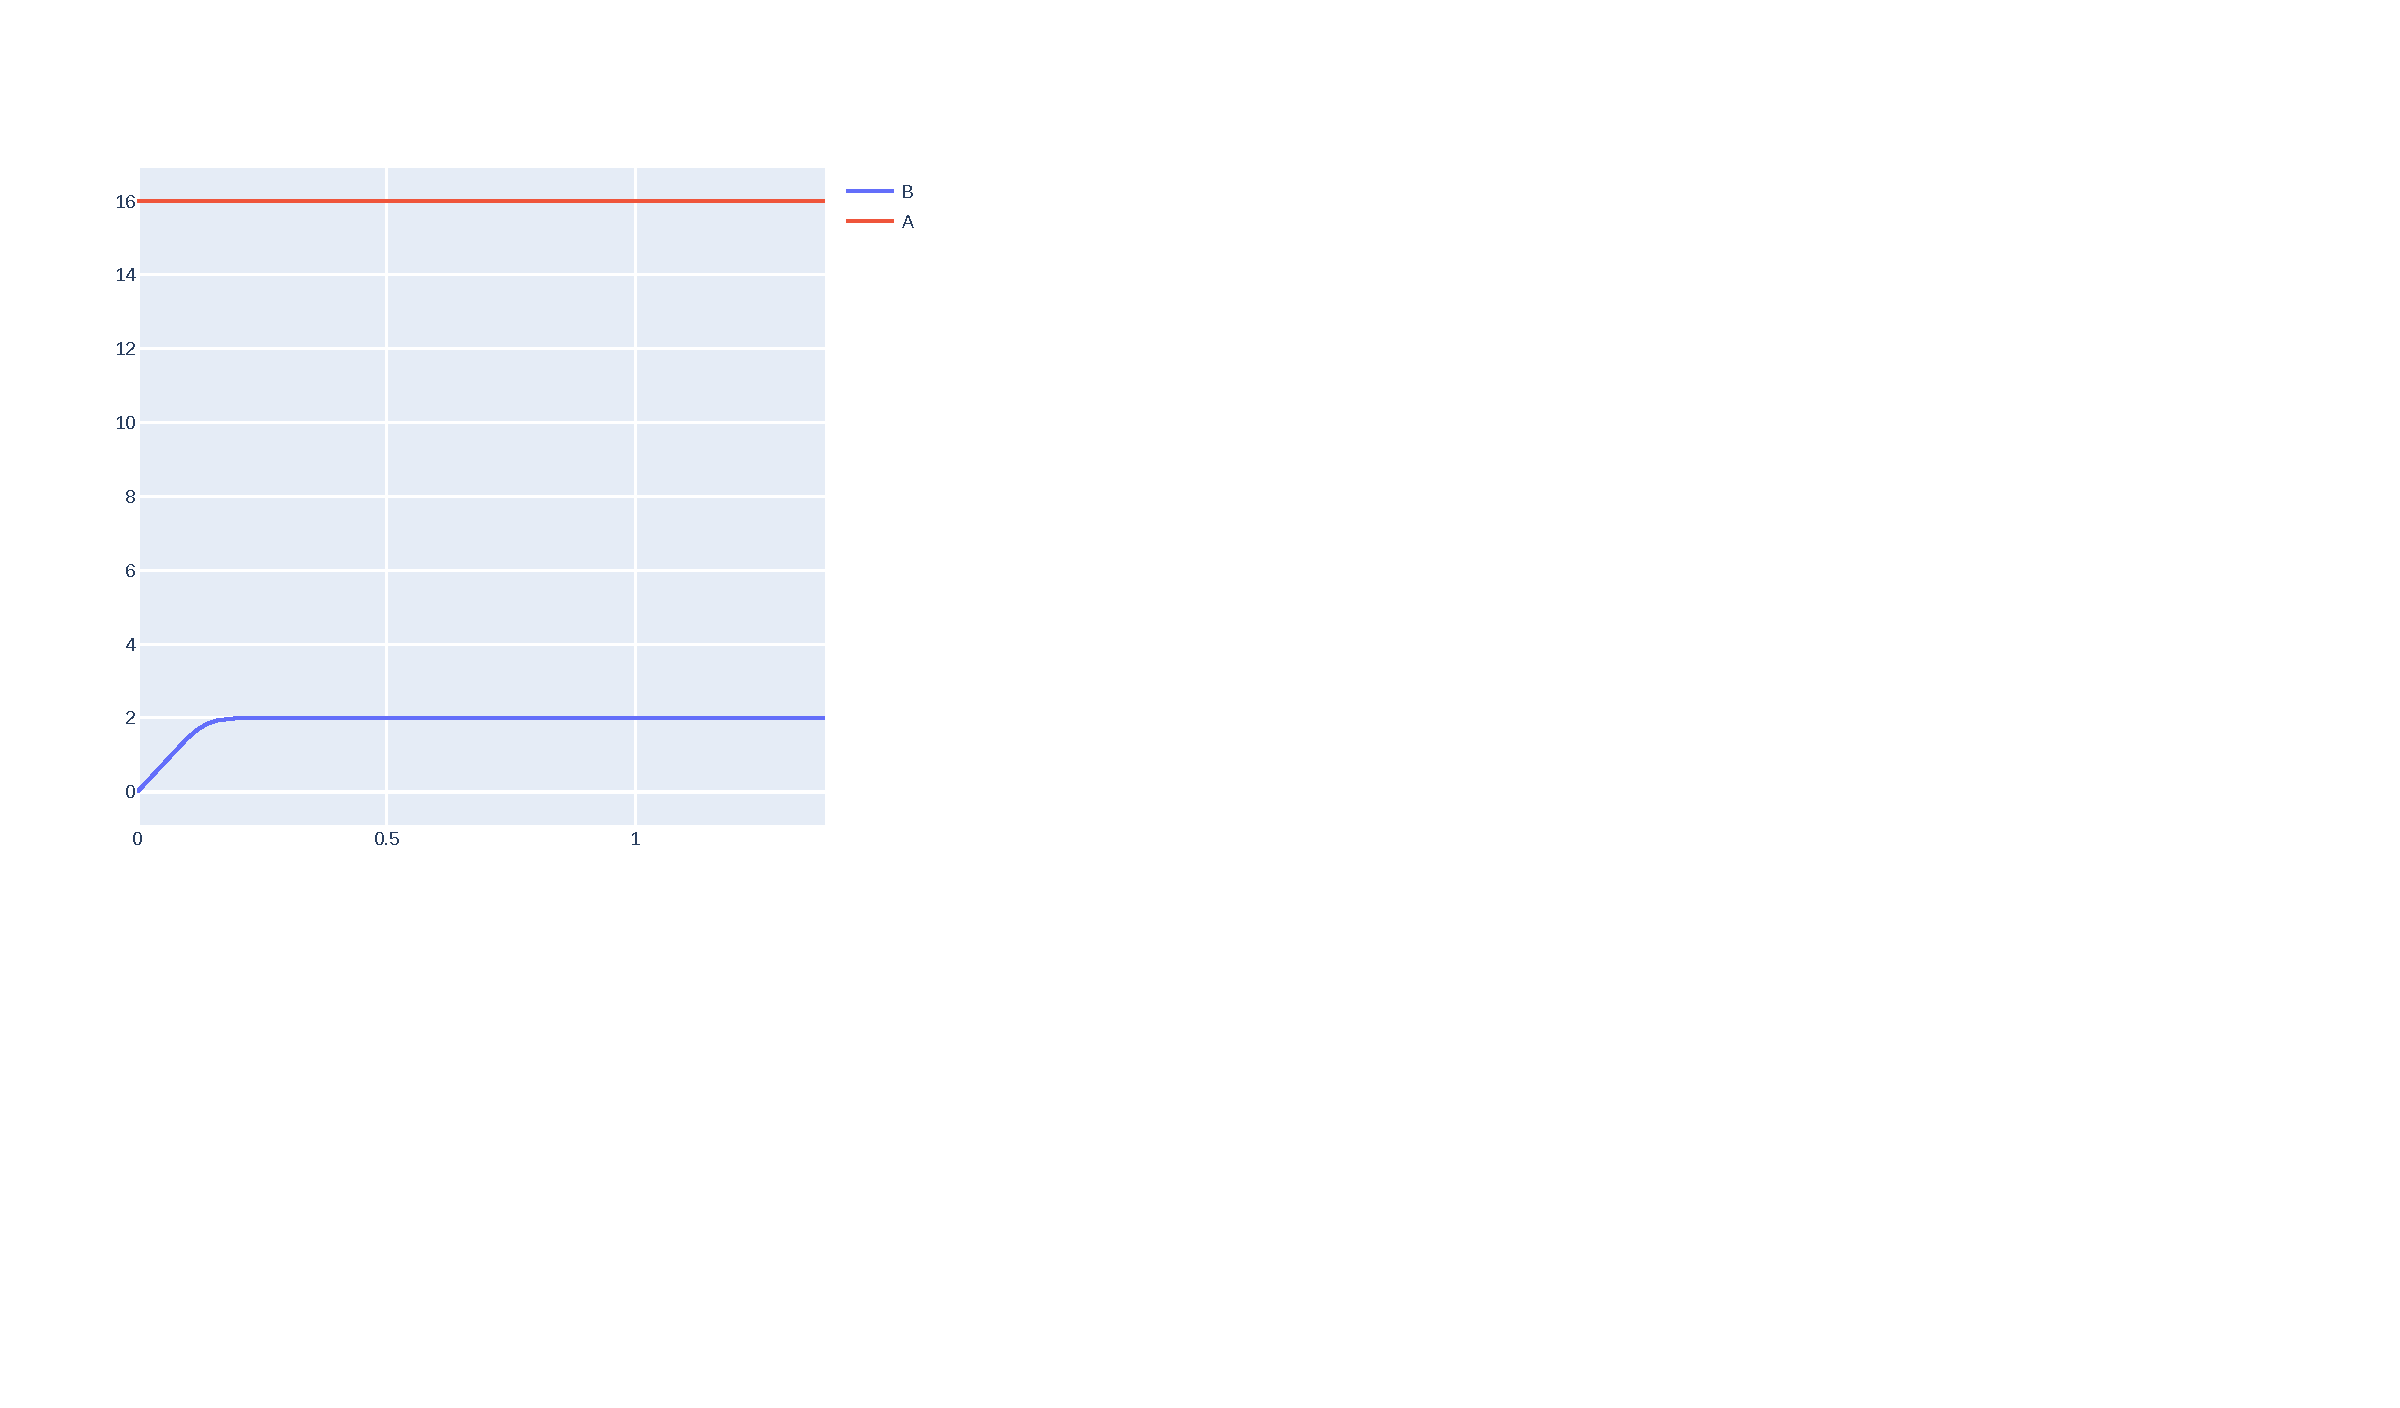
\includegraphics[width=\textwidth]{Figures/sqrt-plot.pdf}
    \caption{\texttt{sqrt[A,B]} resulting in $B=\sqrt[4]{A}$}
    \label{fig:subfigure1}
  \end{subfigure}
  \hfill
  \begin{subfigure}[b]{0.49\textwidth}
    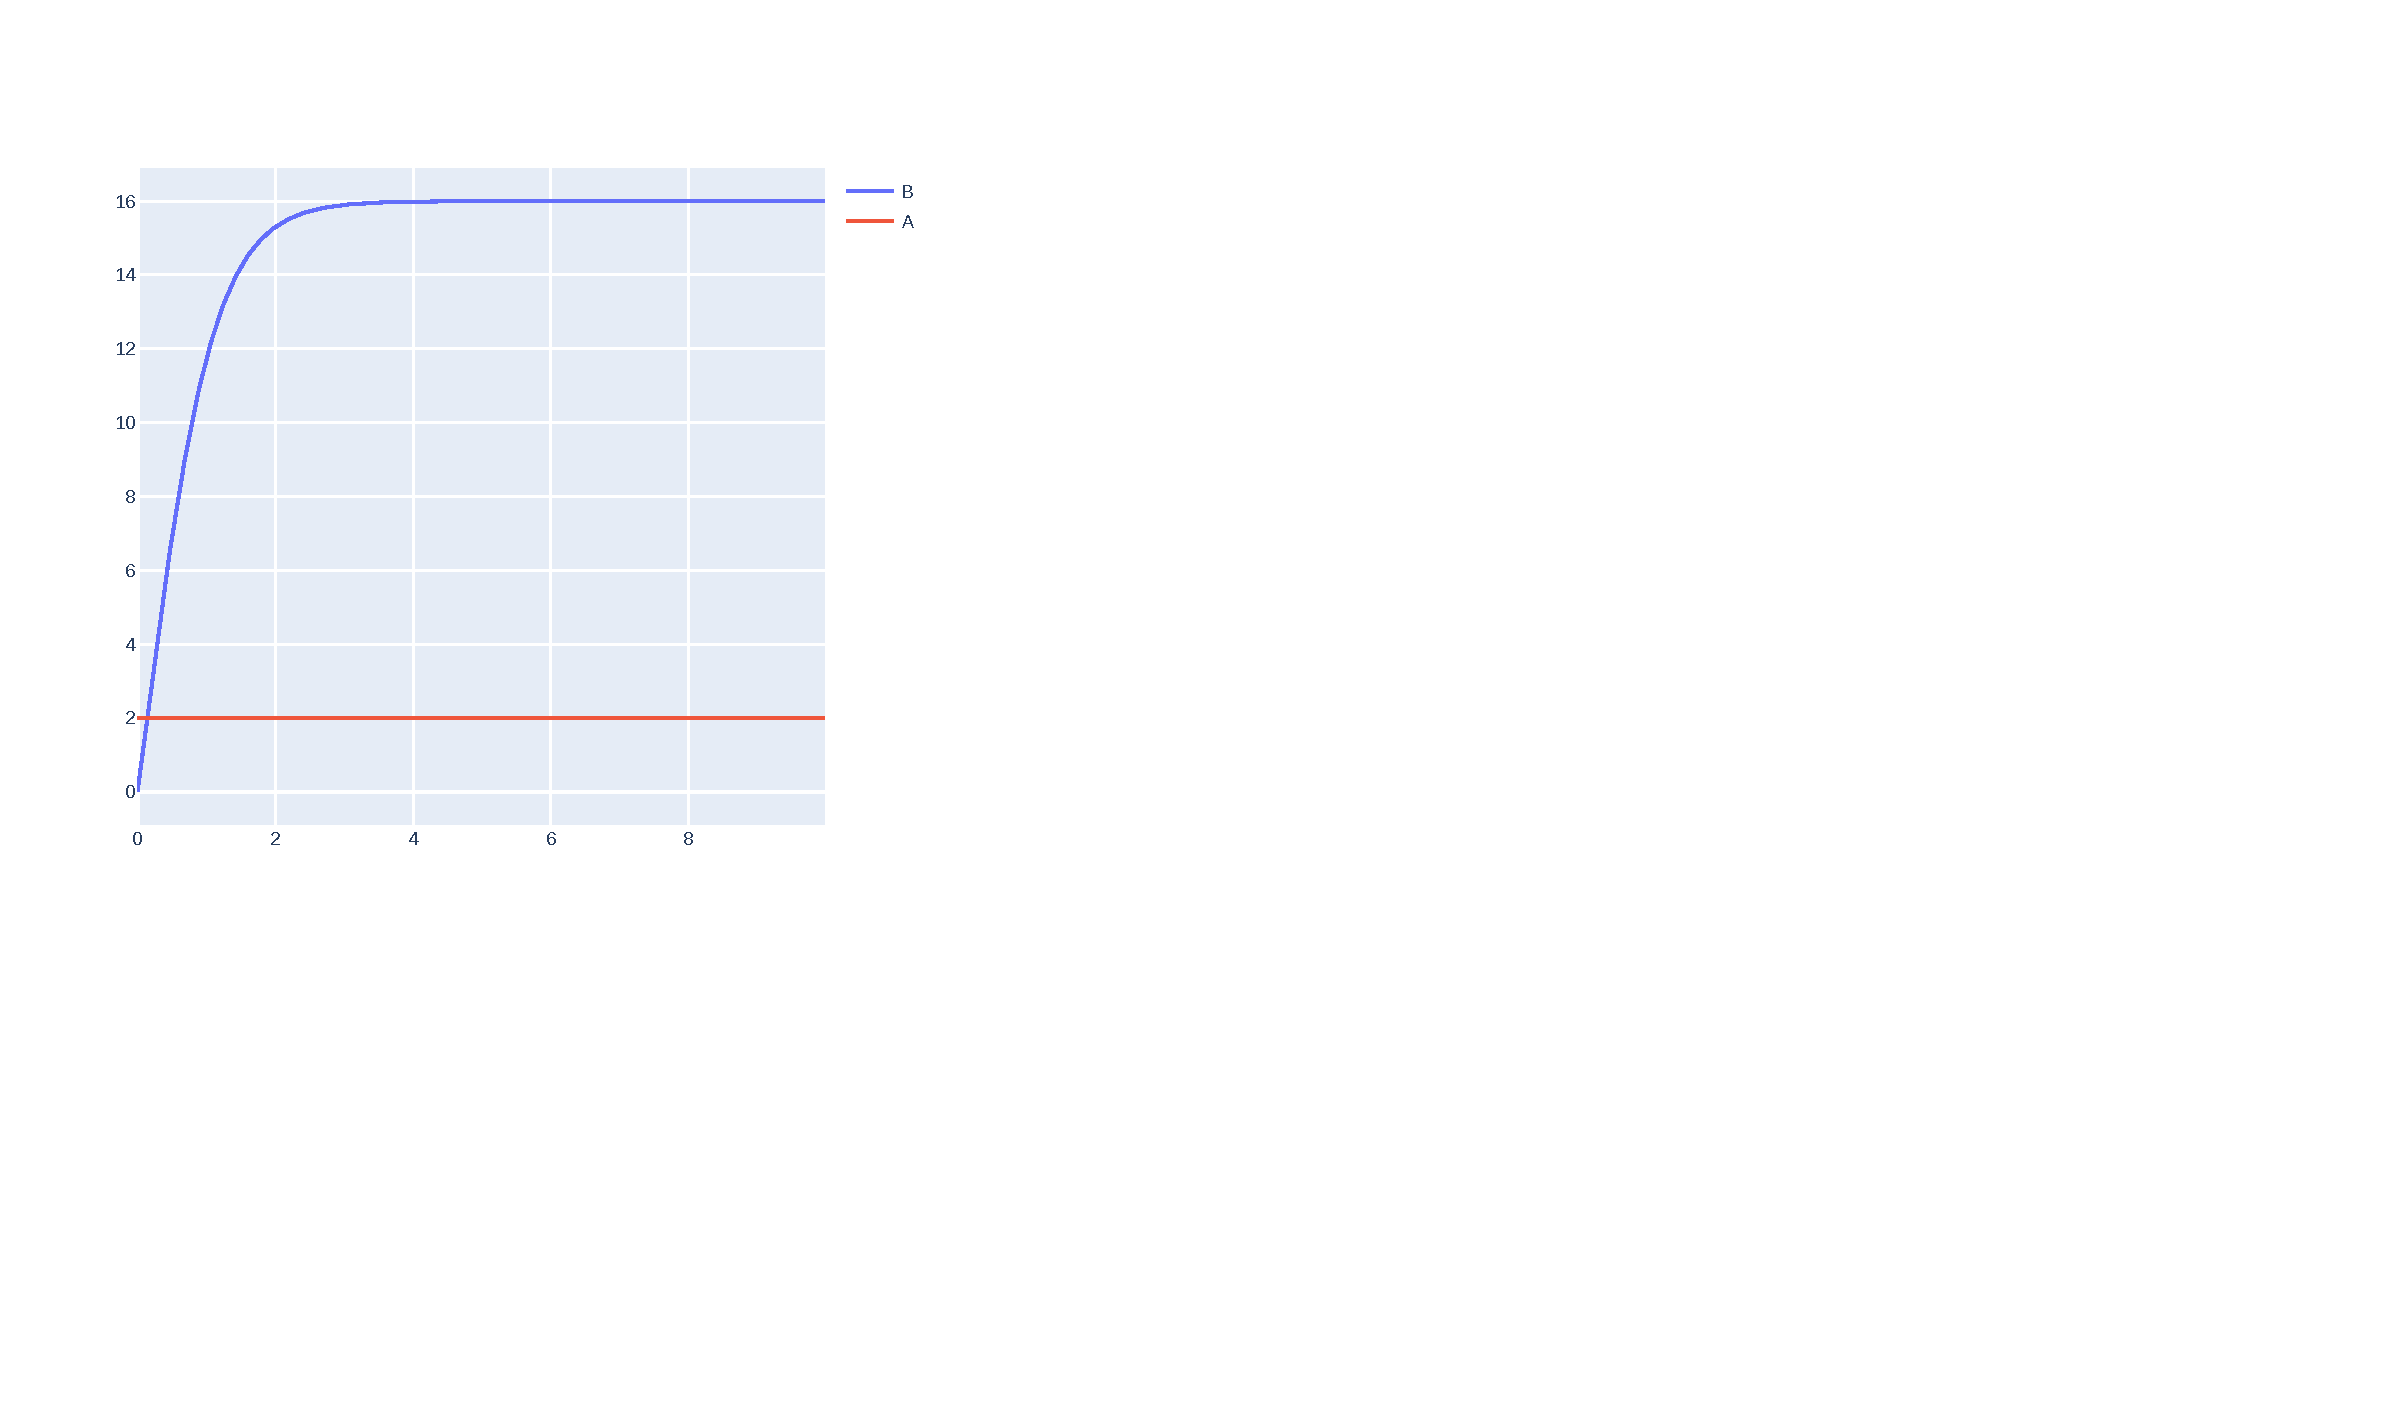
\includegraphics[width=\textwidth]{Figures/mul-plot.pdf}
    \caption{\texttt{mul[A,A,B]} resulting in $B=A^4$}
    \label{fig:subfigure2}
  \end{subfigure}
  \caption{Two showcases of the reaction systems provided in \cite{soloveichik2018a} not providing the correct result.}
  \label{fig:crn-errors}
\end{figure}

Since we have only basic experience in the field of chemistry we resolved to narrowing down our definition of which programs are well-formed such that they do not allow cases where the reactions do not work properly.

One important aspect of this project is the performance of the simulator. We found the simulation to get out of control for $\mathrm{d}t > 0.04\;\mathrm{s}$. With one clock cycle of the chemical oscillators taking around a second, this results in a large number of computations even for shorter simulation runs. We tried to optimize all calculations that are part of the simulation as much as possible. For instance, we chose to evaluate the change of each species in one reaction for each reaction instead of the other way around, since this allows us to reuse the product of all concentrations. Another optimization includes to only calculate concentration changes for non-catalysts, i.e. species which have a none-zero net-change.

The generator we built to generate CRNs, could be further optimized like mentioned earlier by not utilizing filtering by predicates and instead only generating well-formed CRNs by design. Compared to the time required to simulate multiple steps of a CRN, the time used to generate CRNs is negligible since there is basically no perceivable delay in between successive property based testing iterations. 

%Generator does not produce reliable CRN that can be simulated 

\section{Conclusion}
With this project, we have implemented a tool for computation with the CRN++ molecular programming language using functional programming in F\#. We have formulated a revised grammar for CRN++ and a set of \textit{well-formed} properties. 
 
%We have translated the formal properties of trees into F\# predicates that can be tested using property-based testing with the \texttt{FsCheck} package. Also, we have configured \texttt{FsCheck} with classification of test cases, a custom generator and shrinker as well as automated property tests. Furthermore, using our library allows for visualization of the drawing trees as SVG files, with several customizable options. Overall, the project has provided us a great opportunity to familiarize ourselves with coding in F\# as well as the functional paradigm as a whole.

\newpage
\printbibliography


\begin{appendices}
%\chapter*{A}

\section{Revised Grammar}
\begin{Grammar}
\begin{grammar}

<Crn> ::= `crn=\{' <Root> \{`,' <Root> \} `\}' 

<Root> ::= `conc[' <species> `,' <number> `]' \alt `step[' <Command> \{`,' <Command> \} `]'

<Command> ::= <Computation> \alt <Conditional>

<Computation> ::= `rxn[' <Expression> `,' <Expression> `,' <number> `]' \alt <Module>

<Module> ::= `ld[' <species> `,' <species> `]'
\alt `add[' <species> `,' <species> `,' <species> `]'
\alt `sub[' <species> `,' <species> `,' <species> `]'
\alt `mul[' <species> `,' <species> `,' <species> `]'
\alt `div[' <species> `,' <species> `,' <species> `]'
\alt `sqrt[' <species> `,' <species> `]'
\alt `cmp[' <species> `,' <species> `]'

<Conditional> ::= `ifGT[' <Computation> \{ `,' <Computation> \} `]'
\alt `ifGE[' <Computation> \{ `,' <Computation> \} `]'
\alt `ifEQ[' <Computation> \{ `,' <Computation> \} `]'
\alt `ifLT[' <Computation> \{ `,' <Computation> \} `]'
\alt `ifLE[' <Computation> \{ `,' <Computation> \} `]'

<Expression> ::= <species> \{ `+' <species> \}
\end{grammar}
\caption{Revised Grammar for the CRN++ language.}
\label{lst:grammar}
\end{Grammar}

\section{List Parser}
\begin{Grammar}
\begin{grammar}
<ListBlock> ::= <start> <List> <end>

<List> ::= <item> <ItemOpt> \alt $\epsilon$

<ItemOpt> ::= <separator> <item> <ItemOpt> \alt $\epsilon$
\end{grammar}
\caption{The grammar used to parse lists.}
\label{lst:listGrammar}
\end{Grammar}

\newpage

\section{F\# Type Declarations}
\lstinputlisting[
    style=fsharpstyle,
    firstline=7,
    lastline=39,
    caption={F\# type declarations of the main syntactic categories of CRN++ programs.},
    label={lst:crn-types}
]{MolecularProgrammingLib/src/domain/CrnTypes.fs}
\end{appendices}

\end{document}